\section{Potential flow}
\subsection{Irrotational flow}\label{section:IRROTATIONAL}
As mentioned in definition \ref{definition:VP}, one resulting property of the idealisations (steady, inviscid and incompressible flow)
made in this essay is irrotational flow. If flow is rotational, then there exists points at which $\curl{\fatf}\neq0$. In other words, if one were to
imagine a paddle wheel at some point in the fluid, and it spins, then the flow is rotational, and vice versa for irrotational flow.
However, flow being irrotational does not imply that it cannot curve, for example $\curl{\fatf}=0$ in cases such as:
\begin{align*}
    &\fatf:x,y\mapsto X(x,y)\ihat+Y(x,y)\jhat\quad\forall\point{x}{y}\neq\point{0}{0}\\
    &X:x,y\mapsto-\frac{y}{x^2+y^2}\,,\quad Y:x,y\mapsto\frac{x}{x^2+y^2}
\end{align*}
Applying the quotient rule to compute the derivatives for both $X$ and $Y$ gives:
\begin{align*}
    \pdv{X}{y}&=-\frac{\left(\pdv{y}y\right)\left(x^2+y^2\right)-y\pdv{y}\left(x^2+y^2\right)}{\left(x^2+y^2\right)^2}\\
    &=-\frac{x^2+y^2-y(2y)}{\left(x^2+y^2\right)^2}\\
    &=-\frac{x^2-y^2}{\left(x^2+y^2\right)^2}
\end{align*}
\begin{align*}
    \pdv{Y}{x}&=\frac{\left(\pdv{x}x\right)\left(x^2+y^2\right)-x\pdv{x}\left(x^2+y^2\right)}{\left(x^2+y^2\right)^2}\\
    &=\frac{x^2+y^2-x(2x)}{\left(x^2+y^2\right)^2}\\
    &=\frac{-x^2+y^2}{\left(x^2+y^2\right)^2}=-\frac{x^2-y^2}{\left(x^2+y^2\right)^2}
\end{align*}
Thus,
\begin{align*}
    \pdv{X}{y}=\pdv{Y}{x}\implies\pdv{Y}{x}-\pdv{X}{y}=0\\
    \therefore\curl{\fatf}=0
\end{align*}
Plotting the vector field for $\fatf$ reveals circulation around the origin, suggesting rotational flow, but which, with a curl of 0 (everywhere except for
the origin, where $\fatf$ is undefined), is irrotational\referto{figure}{figure:ZEROCURL}.
\begin{figure*}[!ht]
    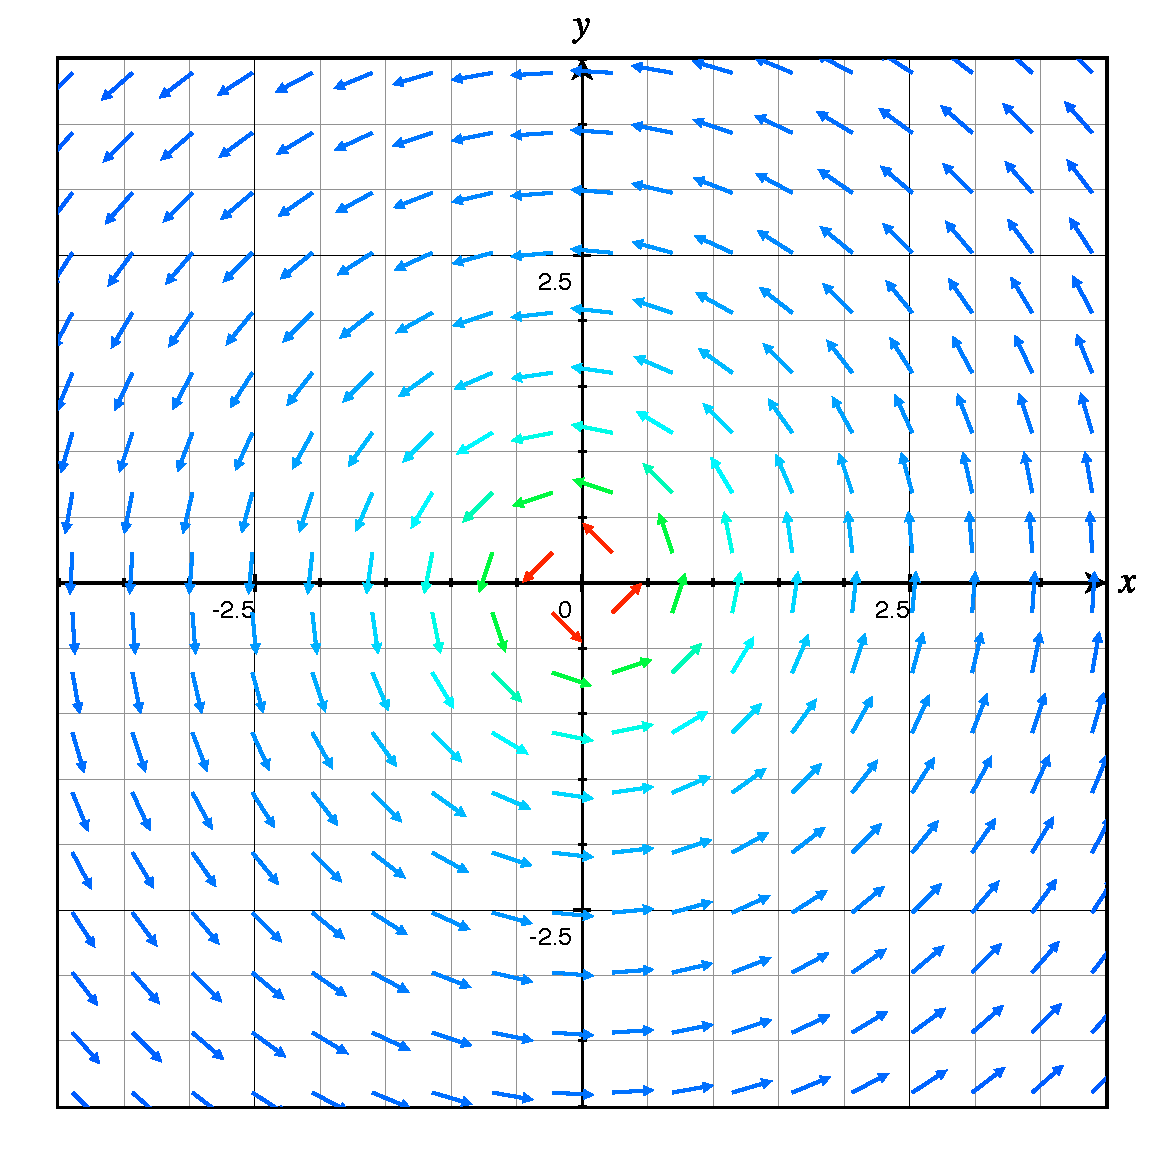
\includegraphics[scale=0.5]{0_curl.pdf}
    \centering
    \caption{The function $\fatf:x,y\mapsto\begin{pmatrix}
        -y\left(x^2+y^2\right)^{-1}\\x\left(x^2+y^2\right)^{-1}
    \end{pmatrix}$ is irrotational despite curving}
    \label{figure:ZEROCURL}
\end{figure*}

\section{Formulation of the problem}
\section{Governing equations and boundary Conditions}